\documentclass{beamer}

\usepackage{default}
\usepackage[utf8]{inputenc}
\usepackage[T1]{fontenc}
%\usepackage[ngerman]{babel}
\usepackage{enumerate}
\usepackage{listings}
\usepackage{marvosym}
\usepackage{gensymb}
\usepackage{graphicx}

\usepackage[nodayofweek]{datetime}
\usepackage{hyperref}
\usepackage{breakurl}


\usepackage{amsmath}
\usepackage{amsfonts}
\usepackage{amssymb}
\usepackage{thmtools}

%\newtheorem{definition}{Definition}
%\newtheorem{proposition}{Propsition}
%\newtheorem{proof}{Proof}
\newtheorem{axiom}{Axiom}



\graphicspath{{./images/}}

\usetheme{metropolis}
%\usecolortheme{beetle}


\title{Trace Link Recovery \\using Static Program Analysis}
\subtitle{\it B.Sc. Thesis Colloquium/Defense}
\author{Maximilian Meffert}
\institute{University of Koblenz-Landau}
\date{$18^{\text{th}}$ January, 2018}

\beamertemplatenavigationsymbolsempty 
\setbeamertemplate{bibliography item}[text]

\makeatother
\setbeamertemplate{footline}[text line]{
\parbox{\linewidth}{
\vspace*{-8pt}
\tiny
\insertshorttitle
\hfill
\insertshortauthor
\hfill
\insertshortinstitute
\hfill
}}
\makeatletter

\newcommand{\Entity}{\textsf{Entity}}
\newcommand{\Artifact}{\textsf{Artifact}}
\newcommand{\File}{\textsf{File}}
\newcommand{\Folder}{\textsf{Folder}}
\newcommand{\Set}{\textsf{Set}}
\newcommand{\Language}{\textsf{Language}}
\newcommand{\Fragment}{\textsf{Fragment}}

\newcommand{\partOf}{\textsf{partOf}}
\newcommand{\properPartOf}{\textsf{properPartOf}}
\newcommand{\atomicPart}{\textsf{atomicPart}}
\newcommand{\fragmentOf}{\textsf{fragmentOf}}
\newcommand{\correspondsTo}{\textsf{correspondsTo}}
\newcommand{\conformsTo}{\textsf{conformsTo}}
\newcommand{\represents}{\textsf{represents}}
\newcommand{\manifestationOf}{\textsf{manifestationOf}}
\newcommand{\sameAs}{\textsf{sameAs}}
\newcommand{\defines}{\textsf{defines}}
\newcommand{\elementOf}{\textsf{elementOf}}

\newcommand{\megal}{\text{MegaL}}
\newcommand{\megalxtext}{\text{MegaL/Xtext}}
\newcommand{\megaltext}{\text{MegaL/Text}}


\definecolor{anti-flashwhite}{rgb}{0.95, 0.95, 0.96}
\lstset{
basicstyle=\tiny,
%morekeywords={company,Company,id},
keywordstyle=\itshape\color{red},
backgroundcolor=\color{anti-flashwhite}
}

\begin{document}

\frame{\titlepage}

\begin{frame}{General Information}
\centering
\textbf{Maximilian Meffert}\\~\\
\resizebox{\textwidth}{!}{
\begin{tabular}{ll}
Mat.-Nr.: & 210 101 205\\
E-Mail: & \href{mailto:maxmeffert@uni-koblenz.de}{maxmeffert@uni-koblenz.de}\\
GitHub: & \url{https://github.com/maxmeffert}\\
Thesis-Repo.: & \url{https://github.com/maxmeffert/BScThesis}
\end{tabular}
}
\\~\vspace{\fill}~\\
\textbf{Supervisors}\\~\\
\resizebox{\textwidth}{!}{
\begin{tabular}{ll}
Prof. Dr. Ralf Lämmel 
& University of Koblenz-Landau, \textit{Institute for Computer Science} \\
M.Sc. Johannes Härtel 
& University of Koblenz-Landau, \textit{Institute for Computer Science}
\end{tabular}
}
\end{frame}

\begin{frame}{In a Nutshell}
\Large
I implemented a system which
\begin{itemize}
\item
recovers \textbf{trace links}
\item
with semantics of \textbf{Linguistic Architectures}
\item
using \textbf{Static Program Analysis} techniques
\end{itemize}
\end{frame}

\begin{frame}[fragile,allowframebreaks]{Motivation: Software as Cognitive Challenge}
\begin{columns}
\begin{column}{0.5\textwidth}
\begin{center}
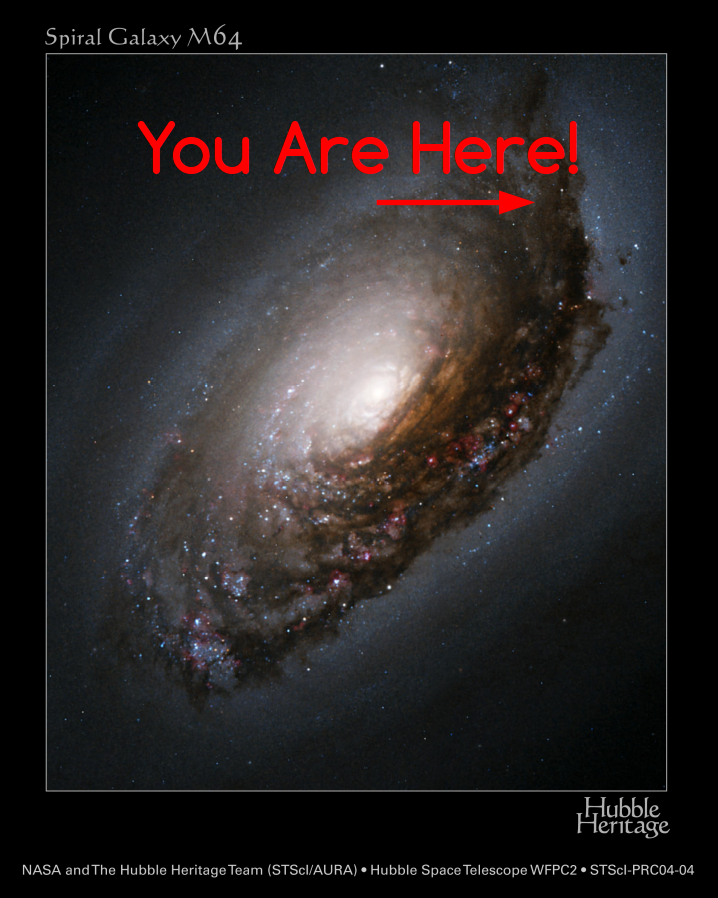
\includegraphics[width=\textwidth]{YouAreHere.png}
\newline
\tiny
View on the "Black Eye" galaxy provided by \cite{BlackEyeGalaxy}.
\end{center}
\end{column}
\begin{column}{0.5\textwidth}
Modern Software Systems are:
\begin{itemize}
\item
large\\(allover artifact count)
\item
heterogeneous\\(languages involved)
\end{itemize}
$\Rightarrow$
challenging for program comprehension tasks 
\end{column}
\end{columns}
\pagebreak
\begin{center}
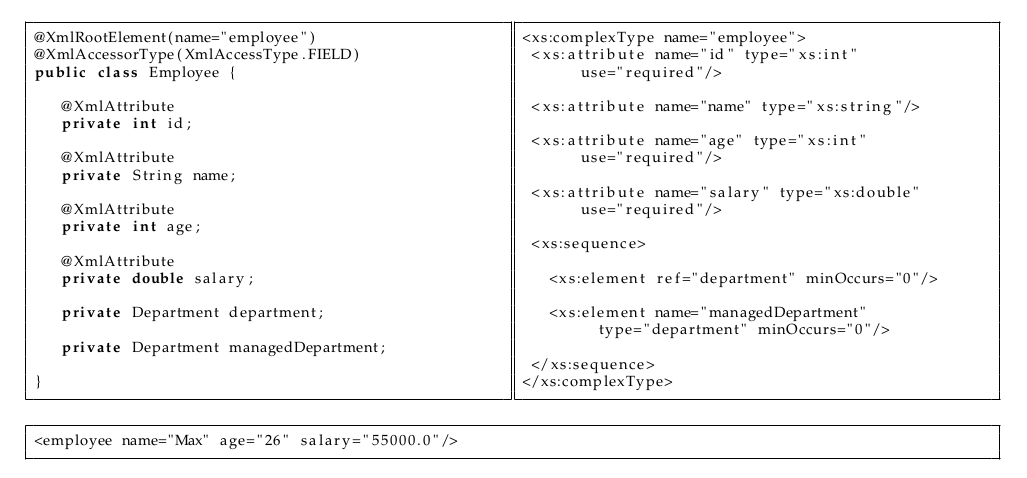
\includegraphics[width=\textwidth]{MotivationalExample.png}
\end{center}
\footnotesize
\begin{itemize}
\item
Structural similarities among Java-, XSD- and XML-files can be observed.
\item
If you are new to a project, you want to know, what belongs together.
\end{itemize}

\end{frame}

\begin{frame}[fragile,allowframebreaks]{Traceability}
We apply \textit{Traceability} as concept supporting program comprehension.
\begin{definition}[Trace]
\begin{description}[align=left]
\item[(Noun)]
A specified triplet of elements comprising: \emph{source artifact}, \emph{target artifact} and a \emph{trace link} associating the two \emph{trace artifacts}. \cite{DBLP:books/daglib/p/GotelCHZEGDAMM12}
\item[(Verb)]
The act of following a trace link. \cite{DBLP:books/daglib/p/GotelCHZEGDAMM12}
\end{description}
\end{definition}
\begin{definition}[Traceability]
The potential for traces to be established and used.
\cite{DBLP:books/daglib/p/GotelCHZEGDAMM12}
\end{definition}

\end{frame}

\begin{frame}[fragile,allowframebreaks]{Linguistic Architectures}
Linguistic Architectures are ...
\begin{itemize}
\item
... the axiomatic study of software systems from software language perspective
\cite{DBLP:conf/modelsward/HeinzLV17}
\cite{DBLP:conf/sle/Lammel16}
\cite{DBLP:conf/ecmdafa/LammelV14}
\cite{DBLP:conf/models/FavreLV12}.

\item
... used to provide semantics for trace links.
\end{itemize}
We want to recover traces with the semantics of axioms for:
\begin{itemize}
\item
$\partOf$,
\item
$\fragmentOf$,
\item
$\correspondsTo$,
\item
and $\conformsTo$ 
\end{itemize}
\pagebreak
\begin{axiom}[partOf]
\begin{align*}
&\partOf(p,w)
\Rightarrow
\Entity(p) \wedge \Entity(w).\\
&\partOf(p,w)
\Leftarrow
p \text{ is a constituent part of } w.
\end{align*}
\end{axiom}

\begin{definition}[porperPartOf]
\begin{align*}
&\properPartOf(p,w)
\Rightarrow
\Entity(p) \wedge \Entity(w).\\
&\properPartOf(x,y)
\Leftarrow
\partOf(x,y) \wedge \neg \partOf(y,x).
\qquad\text{\cite{DBLP:journals/dke/Varzi96} \cite{SEP:Mereology}}
\end{align*}
\end{definition}
\pagebreak
\begin{axiom}[Fragment]
\begin{align*}
&\Fragment(f) 
\Rightarrow
\Artifact(a) \wedge \neg(\File(f) \vee \Folder(f)).\\
&\Fragment(f) 
\Rightarrow 
\exists a.\Artifact(a) \wedge \properPartOf(f,a).
\end{align*}
\end{axiom}

\begin{definition}[fragmentOf]
\begin{align*}
&\fragmentOf(f,x) 
\Rightarrow
\Fragment(f) \wedge \Artifact(x).\\
&\fragmentOf(f,x) 
\Leftarrow
\Fragment(f) \wedge \Artifact(x) \wedge \properPartOf(f,x).
\end{align*}
\end{definition}

\pagebreak
\begin{axiom}[correspondsTo]
Two artifacts representing the same data or information.
\newline
\resizebox{\linewidth}{!}{
\begin{minipage}{\linewidth}
\begin{align*}
\correspondsTo(x,y)
&\Rightarrow
\Artifact(x) \wedge \Artifact(y).\\
\correspondsTo(x,y)
&\Leftarrow
(\forall px.\properPartOf(px,x) \Rightarrow \exists py.\properPartOf(py,y) \wedge \correspondsTo(px,py))\\
&\wedge
(\forall py.\properPartOf(py,y) \Rightarrow \exists px.\properPartOf(px,x) \wedge \correspondsTo(py,px))\\
&\vee
(\not\exists p.\properPartOf(p,x) \vee \properPartOf(p,y)) \wedge \sameAs(x,y).
\end{align*}
\end{minipage}
}
\end{axiom}
\begin{axiom}[conformsTo] 
Two artifacts where one defines the other.
\newline
\resizebox{\linewidth}{!}{
\begin{minipage}{\linewidth}
\begin{align*}
\conformsTo(a,d)
&\Rightarrow
\Artifact(a) \wedge \Artifact(d).\\
\conformsTo(a,d)
&\Leftarrow
(\forall pa.\properPartOf(pa,a) \wedge \exists pd.\properPartOf(pd,d) \wedge \conformsTo(pa,pd))\\
&\vee \exists l.\defines(d,l) \wedge \elementOf(a,l).
\end{align*}
\end{minipage}
}
\end{axiom}
\end{frame}

\begin{frame}[fragile,allowframebreaks]{Trace Link Recovery Approach}
\begin{center}
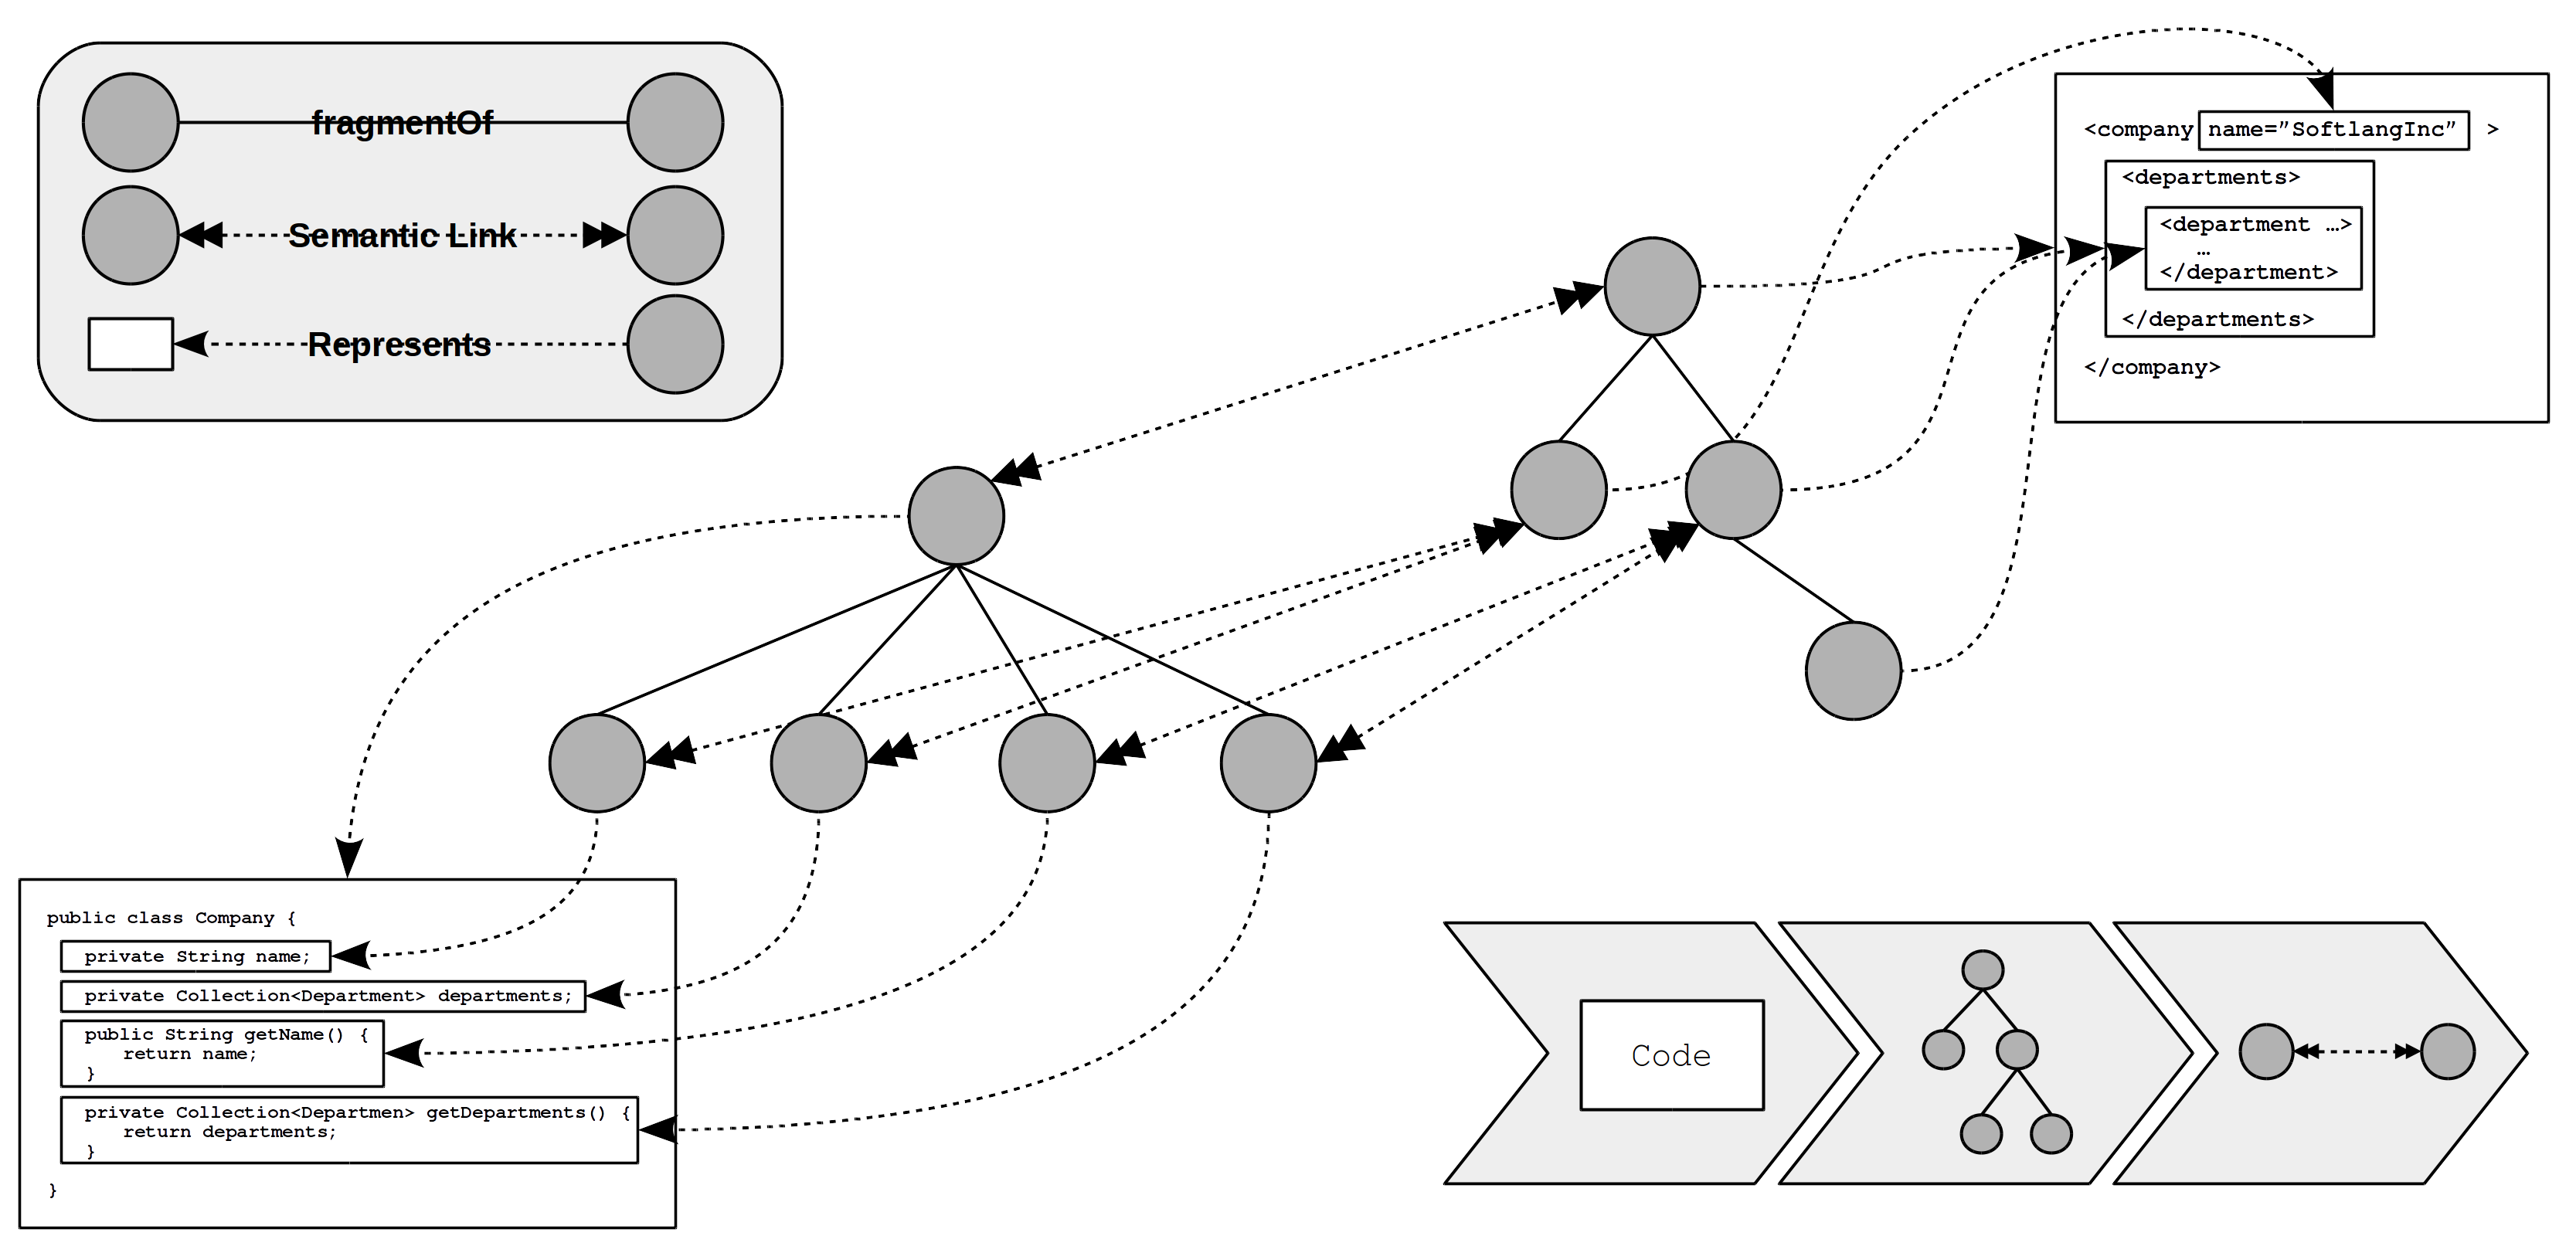
\includegraphics[width=\textwidth]{RecoveryApproach.png}
\end{center}
\pagebreak
Trace Link Recovery Process
\begin{center}
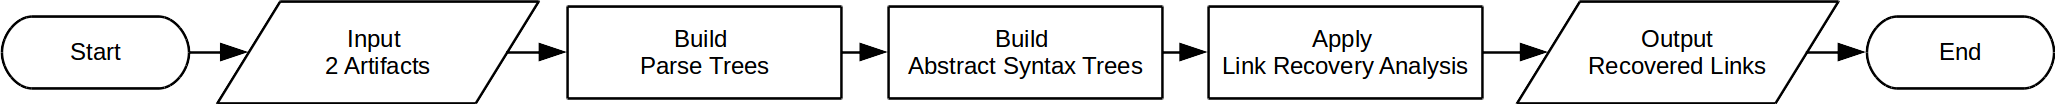
\includegraphics[width=\textwidth]{RecoveryProcess.png}
\end{center}
\begin{enumerate}
\item
Create two Parse Trees from both inputs respectively.
\item
Both Parse Trees are transformed to Abstract Syntax Trees supporting analysis of the represented contents.
\item
Comparative Analysis of both Abstract Syntax Trees:
while traversing through both trees we check whether each pair of nodes is a trace link.
\end{enumerate}
\end{frame}

\begin{frame}[fragile,allowframebreaks]{Trace Link Recovery System}
\begin{center}
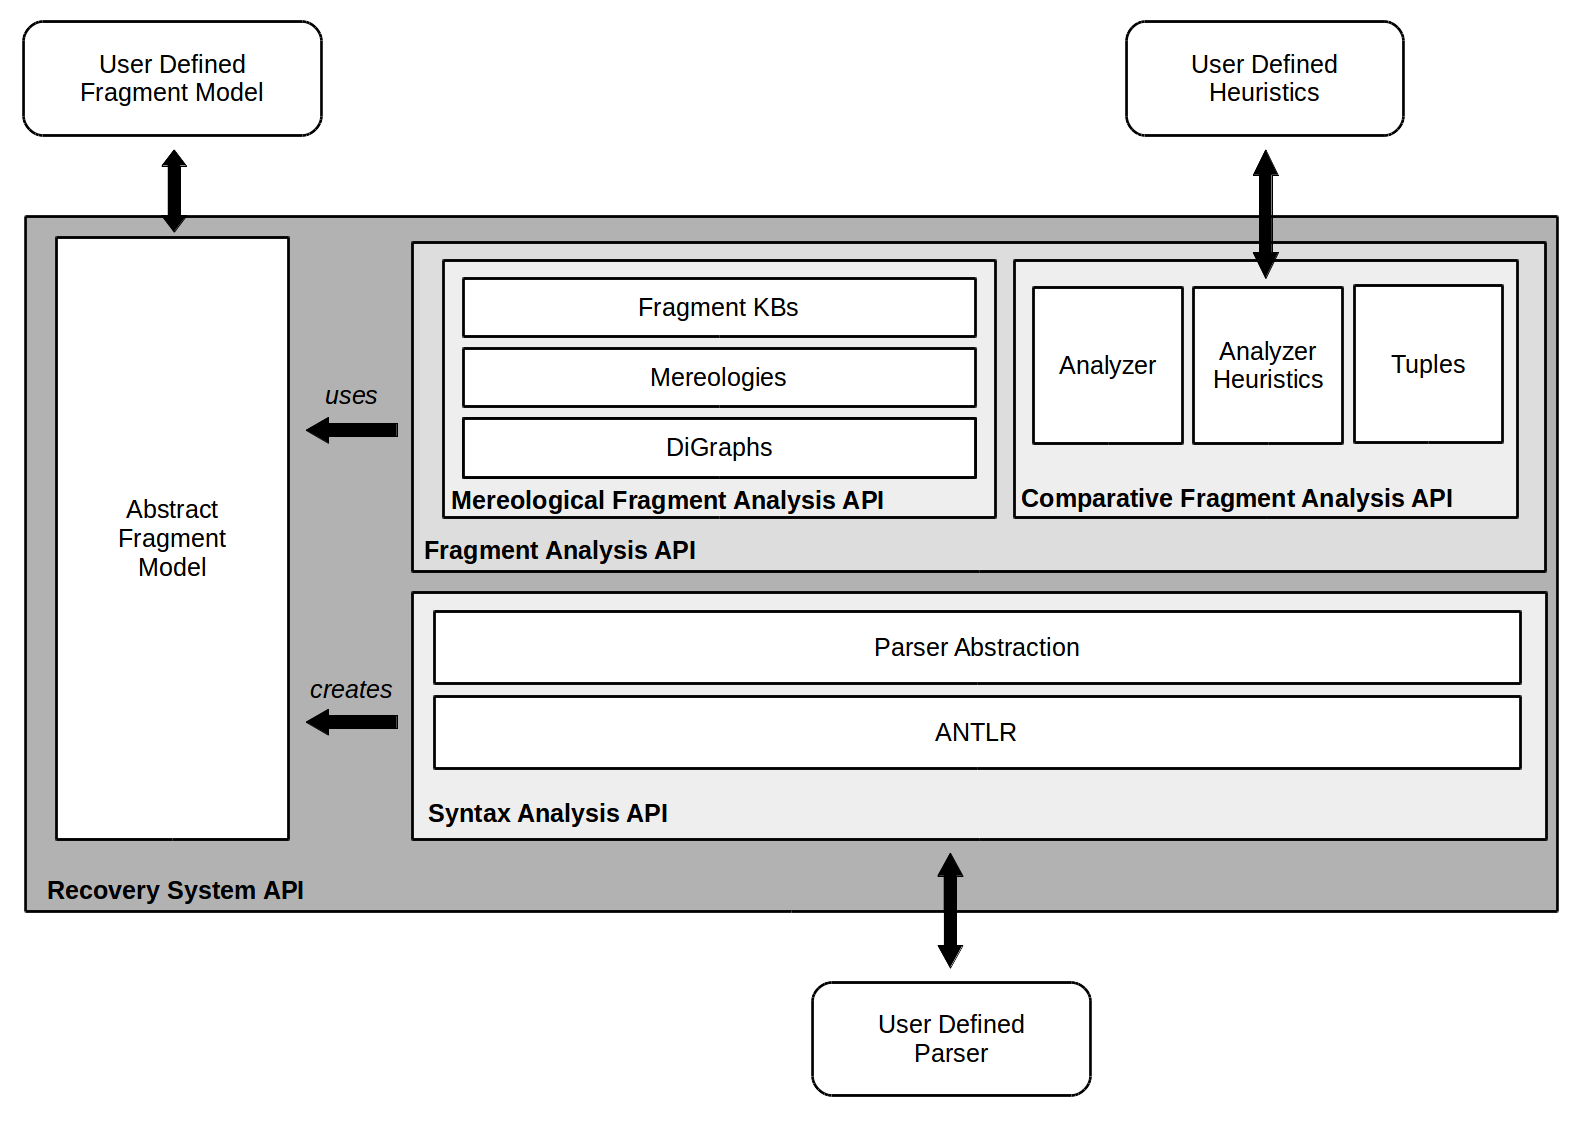
\includegraphics[width=.8\textwidth]{RecoverySystemAPI.png}
\\
\textbf{Recovery System API}
\end{center}
\pagebreak
\begin{center}
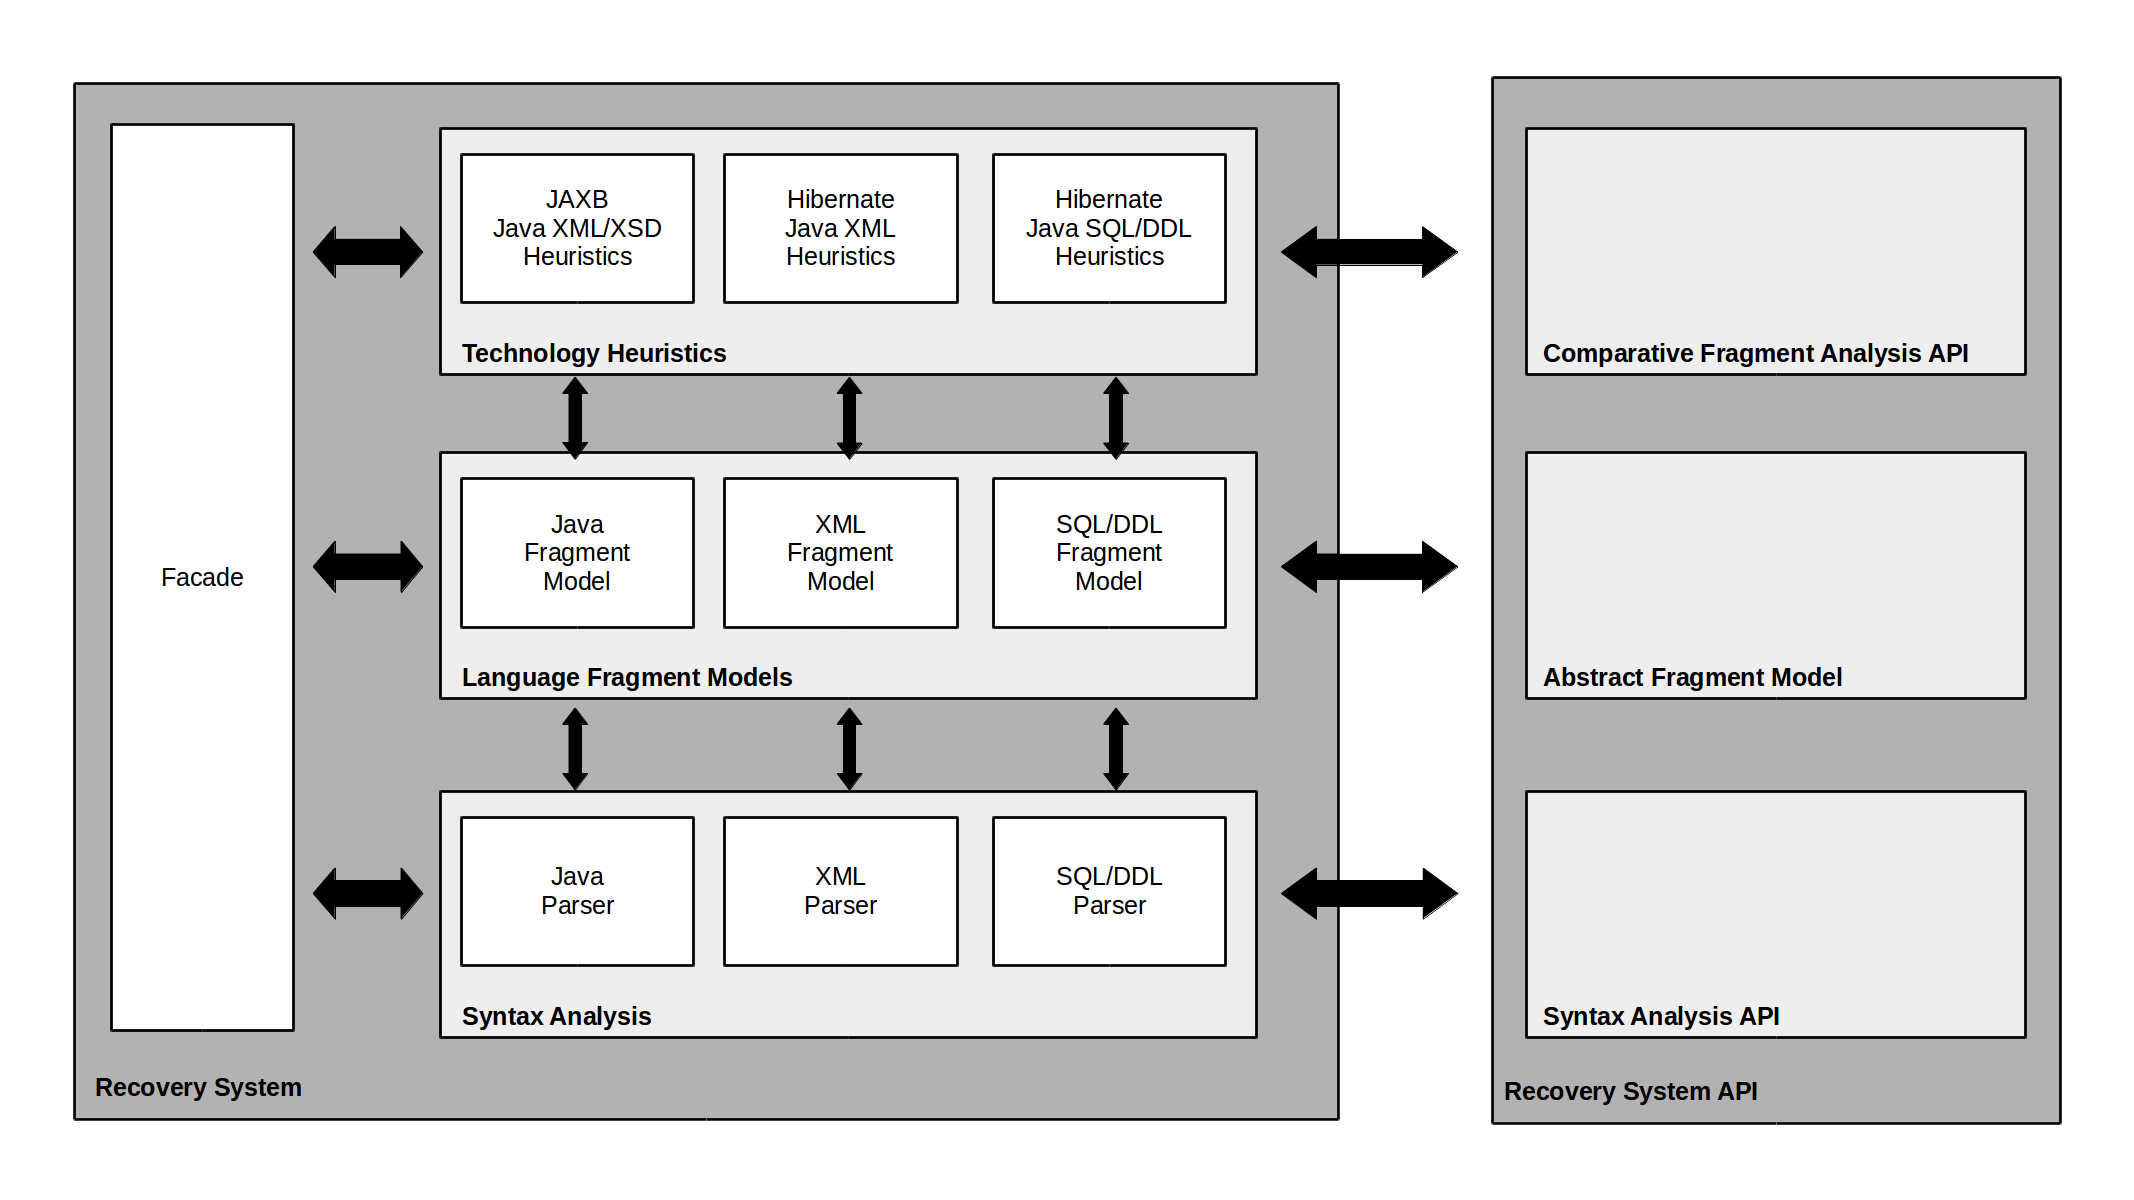
\includegraphics[width=.9\textwidth]{RecoverySystem.png}
\\
\textbf{Recovery System}
\end{center}
\pagebreak
\begin{center}
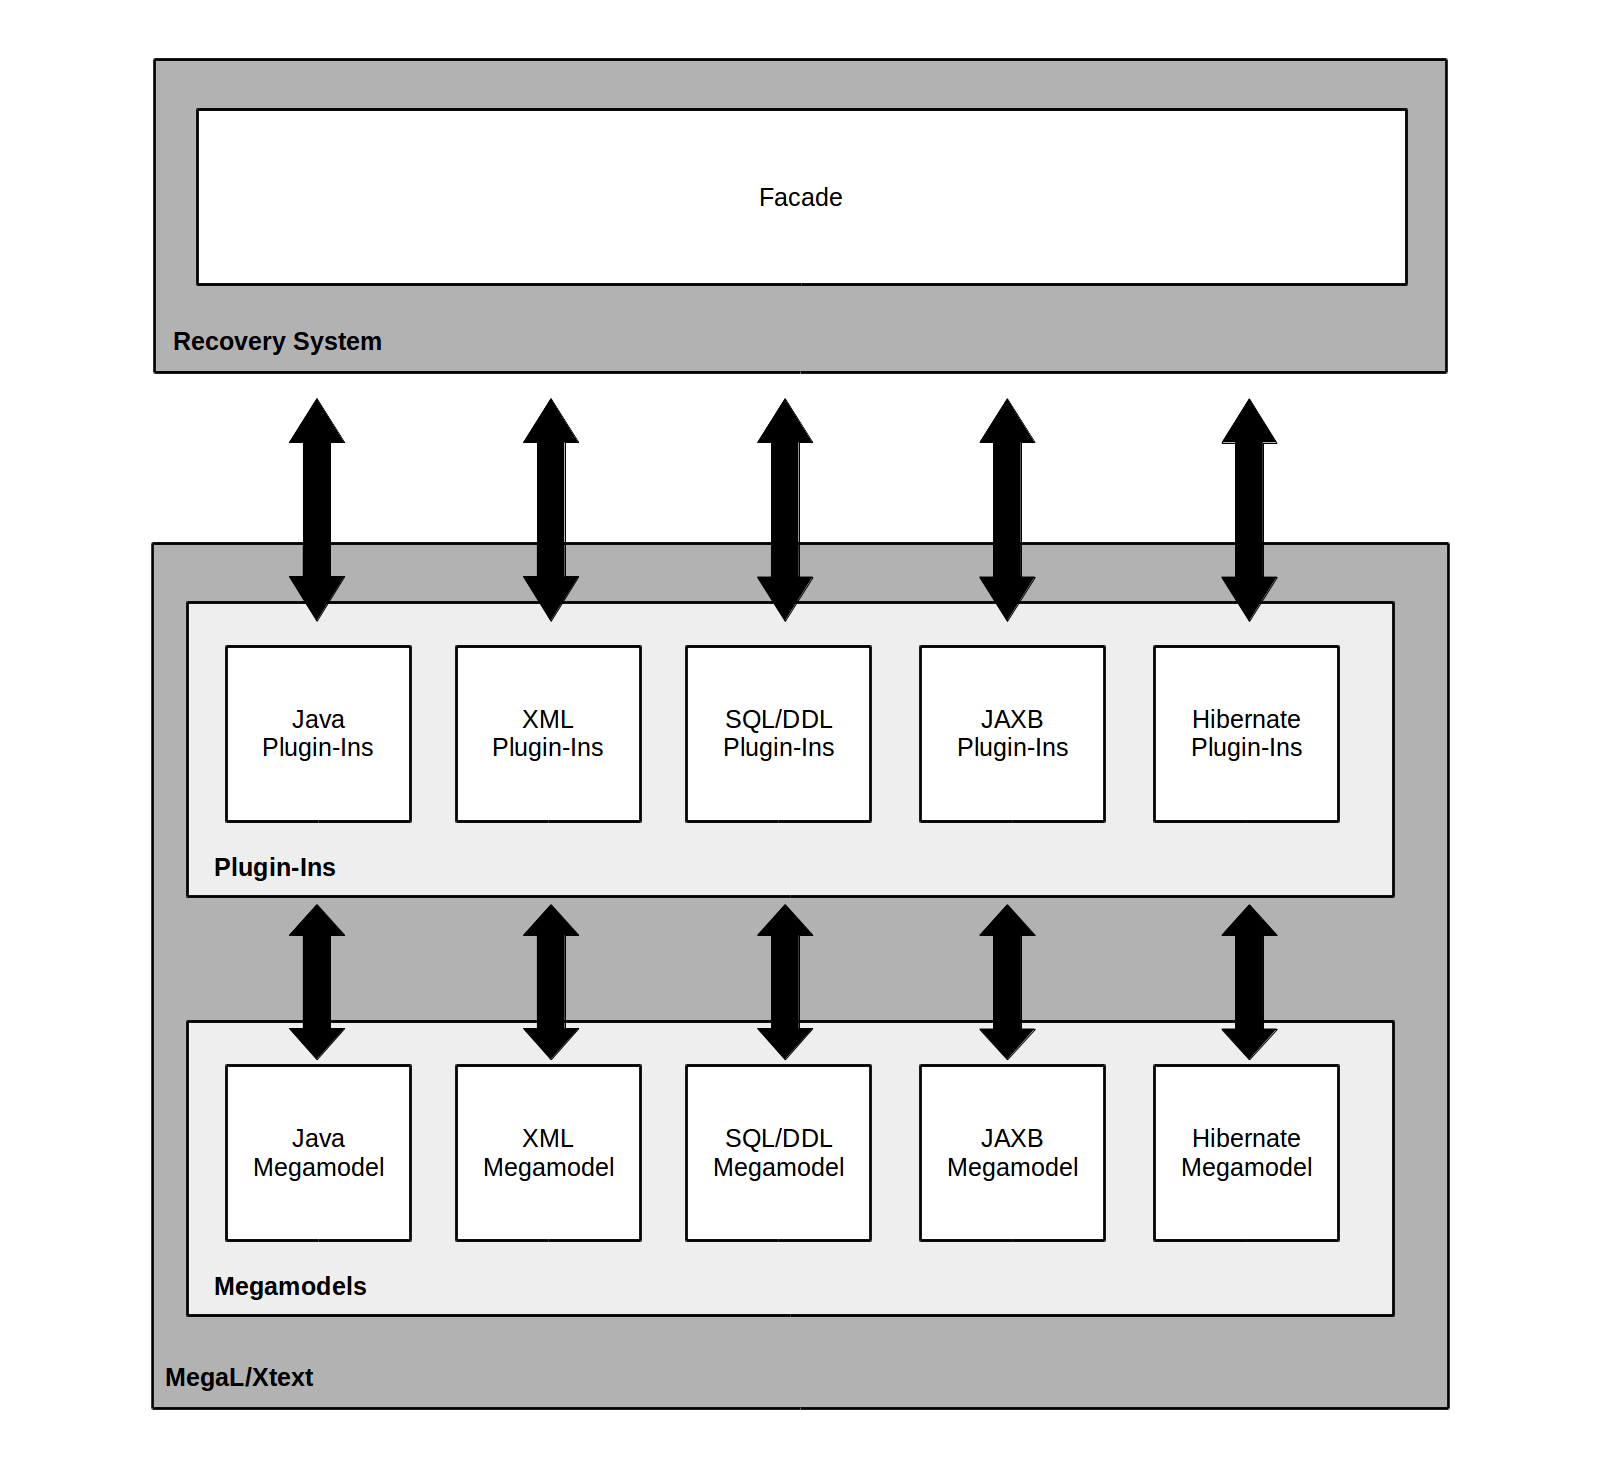
\includegraphics[width=.7\textwidth]{MegalXtextIntegrationDesign.png}
\\
\textbf{Integration into \megalxtext}
\end{center}
\end{frame}

\begin{frame}[fragile,allowframebreaks]{Mini Case Study}
\begin{itemize}
\item
Evaluates whether the Recovery Systems preserves semantics of Linguistic Architectures.
\item
Uses a JAXB and Hibernate implementation of the 101companies HRMS model as corpus.
\end{itemize}
\begin{center}
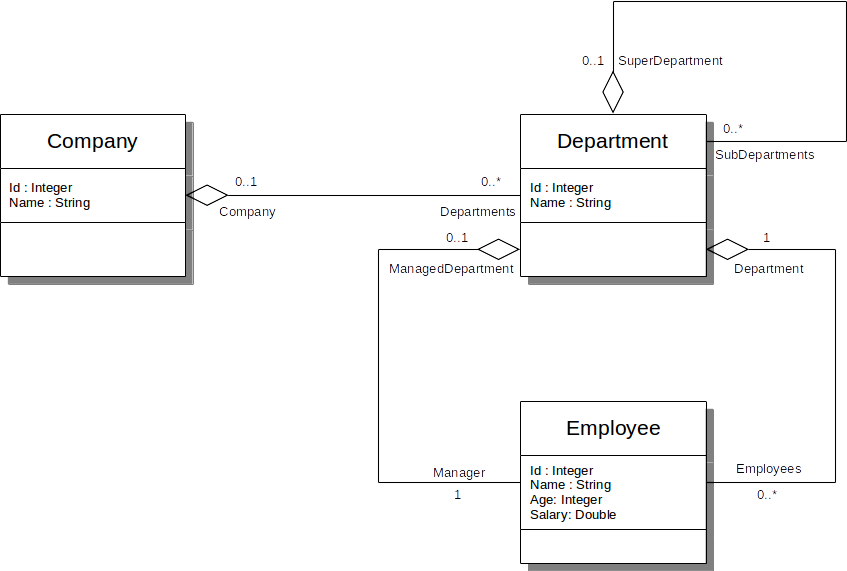
\includegraphics[width=.5\textwidth]{101HRMSModel.png}
\\
\url{https://101wiki.softlang.org/101:@system}
\end{center}
\pagebreak
\textbf{Setup (1)}
\begin{lstlisting}
companyJavaFile : File
companyJavaFile = '/input/Company.java'

companyHbmFile : File
companyHbmFile = '/input/Company.hbm.xml'

departmentJavaFile : File
departmentJavaFile = '/input/Department.java'

departmentHbmFile : File
departmentHbmFile = '/input/Department.hbm.xml'

employeeJavaFile : File
employeeJavaFile = '/input/Employee.java'

employeeHbmFile : File
employeeHbmFile = '/input/Employee.hbm.xml'

companiesXmlFile: File
companiesXmlFile = '/input/companies.xml'

companiesXsdFile: File
companiesXsdFile = '/input/companies.xsd'

comaniesSqlFile : File
comaniesSqlFile = '/input/companies.ddl.sql'
\end{lstlisting}
\pagebreak
\textbf{Setup (2)}
\begin{lstlisting}
companyJavaFile correspondsTo companiesXsdFile
companyJavaFile correspondsTo comaniesSqlFile
companyJavaFile correspondsTo companyHbmFile

departmentJavaFile correspondsTo companiesXsdFile
departmentJavaFile correspondsTo comaniesSqlFile
departmentJavaFile correspondsTo departmentHbmFile

employeeJavaFile correspondsTo companiesXsdFile
employeeJavaFile correspondsTo comaniesSqlFile
employeeJavaFile correspondsTo employeeHbmFile

companiesXmlFile conformsTo companiesXsdFile
\end{lstlisting}
\pagebreak
\begin{center}
\textbf{Absolute Metrics}
\begin{align*}
\#\Artifact &:= |\{ x : \Artifact(x) \}| \\
\#\File &:= |\{ x : \File(x) \}| \\
\#\Fragment &:= |\{ x : \Fragment(x) \}|\\
\#\partOf &:= |\{ (x,y) : \partOf(x,y) \}| \\
\#\fragmentOf &:= |\{ (x,y) : \fragmentOf(x,y) \}| \\
\#\correspondsTo &:= |\{ (x,y) : \correspondsTo(x,y) \}| \\
\#\conformsTo &:= |\{ (x,y) : \conformsTo(x,y) \}| 
\end{align*}
\end{center}
\pagebreak
\begin{center}
\textbf{Relative Metrics}
\begin{align*}
\#\partOf(x) &:= |\{ y : \partOf(y,x) \}| \\
\#\fragmentOf(x) &:= |\{ y : \fragmentOf(y,x) \}| \\
\#\correspondsTo(y) &:=
|\{ x : \correspondsTo(x,y') \wedge \fragmentOf(y',y)  \}|
\\
\#\conformsTo(y) &:=
|\{ x : \conformsTo(x,y') \wedge \fragmentOf(y',y)  \}|\\
\#LHS(R) &:= |\{ x : R(x,y) \}| \\
\#RHS(R) &:= |\{ y : R(x,y) \}| 
\end{align*}
\end{center}
\pagebreak
\begin{center}
\begin{tabular}{|l|l|l|}
\hline
$\#\Artifact$ & $\#\File$ & $\#\Fragment$
\\ \hline
483 & 9 & 474 
\\ \hline
\end{tabular}

\begin{tabular}{|l|l|l|l|}
\hline
$\#\partOf$ & $\#\fragmentOf$ & $\#\correspondsTo$ & $\#\conformsTo$
\\ \hline
1847 & 1837 & 106 & 81 
\\ \hline
\end{tabular}
\end{center}
\begin{itemize}
\item
$\#\Artifact = \#\File + \#\Fragment$
\item
$\#\partOf = \#\fragmentOf + 10$ (due to \megalxtext plug-in configuration)
\end{itemize}
\pagebreak
\begin{center}
\tiny
\begin{tabular}{|l|l|l|}
\hline
$x$ & $\#\partOf(x)$ & $\#\fragmentOf(x)$
\\ \hline
companyJavaFile & 9 & 9 
\\ \hline
companyHbmFile & 51 & 51 
\\ \hline
departmentJavaFile & 20 & 20 
\\ \hline
departmentHbmFile & 112 & 112 
\\ \hline
employeeJavaFile & 15 & 15 
\\ \hline
employeeHbmFile & 76 & 76 
\\ \hline
companiesXmlFile & 89 & 89 
\\ \hline
companiesXsdFile & 85 & 85 
\\ \hline
comaniesSqlFile & 17 & 17 
\\ \hline \hline
\textbf{Sum:} & 474 & 474 
\\ \hline 
\end{tabular}
\end{center}
\begin{itemize}
\item
$\forall x. \#\partOf(x) = \#\fragmentOf(x)$
\item
$\#\Fragment = \sum\limits_{x} \#\fragmentOf(x)$
\end{itemize}
$\Rightarrow$
Indicates, each fragment is indeed a part.
\pagebreak
\begin{center}
\tiny
\begin{tabular}{|l|l|l|}
\hline
$x$ & $\#\correspondsTo(x)$ & $\#\conformsTo(x)$
\\ \hline
companyJavaFile & 12 & 0 
\\ \hline
companyHbmFile & 4 & 0 
\\ \hline
departmentJavaFile & 15 & 0 
\\ \hline
departmentHbmFile & 5 & 0 
\\ \hline
employeeJavaFile & 17 & 0 
\\ \hline
employeeHbmFile & 5 & 0 
\\ \hline
companiesXmlFile & 0 & 0 
\\ \hline
companiesXsdFile & 16 & 67 
\\ \hline
comaniesSqlFile & 11 & 0 
\\ \hline 
\end{tabular}
\end{center}
\begin{itemize}
\item
$x \neq \text{companiesXsdFile} \Rightarrow \#\conformsTo(x) = 0$
\item
$\#\correspondsTo(\text{companiesXmlFile}) = 0$ 
\end{itemize}
$\Rightarrow$
Indicates no correspondence between model- and instance-level entities.
Vice versa, conformance only occurs between model- and instance-level entities.
\pagebreak
\begin{center}
\begin{tabular}{|l|l|l|}
\hline
$R$ & $\#LHS(R)$ & $\#RHS(R)$
\\ \hline
$\partOf$ & 484 & 121
\\ \hline
$\fragmentOf$ & 474 & 117
\\ \hline
$\correspondsTo$ & 68 & 68
\\ \hline
$\conformsTo$ & 68 & 19
\\ \hline 
\end{tabular}
\end{center}
\begin{itemize}
\item
$\#LHS(\correspondsTo) = \#RHS(\correspondsTo)$
\end{itemize}
$\Rightarrow$
Indicates correspondence is a bijection as postulated.
\end{frame}

\begin{frame}[fragile,allowframebreaks]{References}
\bibliographystyle{splncs}
\bibliography{bibliography}{}
\end{frame}


\end{document}
